\documentclass[11pt,a4paper]{article}

\usepackage[utf8]{inputenc}
\usepackage[T1]{fontenc}
\usepackage[spanish,es-nodecimaldot]{babel}
\usepackage{lmodern}
\usepackage{microtype}
\usepackage{geometry}
\usepackage{graphicx}
\usepackage{booktabs}
\usepackage{tabularx}
\usepackage{array}
\usepackage{float}
\usepackage[table]{xcolor}
\usepackage{hyperref}
\usepackage{fancyhdr}
\usepackage{listings}
\usepackage{caption}

\geometry{top=22mm,bottom=23mm,left=23mm,right=23mm}
\graphicspath{{diagrams/}{evidence/}}
\setlength{\parindent}{0pt}
\setlength{\parskip}{0.55em}

\definecolor{fpgaBlue}{HTML}{1D4ED8}
\definecolor{configGreen}{HTML}{059669}
\definecolor{txOrange}{HTML}{D97706}
\definecolor{rxViolet}{HTML}{7C3AED}
\definecolor{lightGray}{HTML}{F3F4F6}
\definecolor{textGray}{HTML}{374151}

\hypersetup{
    colorlinks=true,
    linkcolor=fpgaBlue,
    urlcolor=fpgaBlue,
    pdftitle={Controlador FPGA para transceptor LoRa SX1278},
    pdfsubject={Trabajo final de Circuitos Lógicos Programables}
}

\pagestyle{fancy}
\setlength{\headheight}{14pt}
\fancyhf{}
\lhead{Controlador FPGA para LoRa SX1278}
\rhead{Trabajo final}
\cfoot{\thepage}
\renewcommand{\headrulewidth}{0.4pt}

\captionsetup{font=small,labelfont=bf}

\lstset{
    basicstyle=\ttfamily\small,
    backgroundcolor=\color{lightGray},
    frame=single,
    rulecolor=\color{gray!35},
    breaklines=true,
    columns=fullflexible,
    showstringspaces=false
}

\newcommand{\module}[1]{\texttt{#1}}

\begin{document}

\pagenumbering{gobble}
\begin{titlepage}
    \centering
    \vspace*{18mm}
    {\color{fpgaBlue}\rule{\textwidth}{1.4pt}}\\[13mm]
    {\Huge\bfseries Controlador FPGA para transceptor LoRa SX1278\par}
    \vspace{5mm}
    {\Large Interfaz UART, controlador SPI y gestión de CONFIG, TX y RX\par}
    \vspace{13mm}
    {\color{fpgaBlue}\rule{\textwidth}{1.4pt}}

    \vfill
    {\Large Circuitos Lógicos Programables\par}
    \vspace{4mm}
    {\large Trabajo práctico final\par}
    \vspace{16mm}
    {\large Plataforma: Zybo Zynq-7000\par}
    {\large Periférico: SX1278, 433 MHz\par}
    \vfill
    {\large 4to bimestre de 2026\par}
\end{titlepage}

\pagenumbering{roman}
\tableofcontents
\clearpage
\pagenumbering{arabic}

\section{Introducción}

El trabajo implementa en VHDL un controlador para el transceptor LoRa SX1278
sobre una placa Zybo Zynq-7000. El sistema recibe órdenes desde una PC mediante
UART, las interpreta y genera las transacciones SPI necesarias para configurar
el transceptor, transmitir payloads y recuperar paquetes recibidos.

La naturaleza del producto es la de un \textbf{módem LoRa serie}: el equipo
host intercambia comandos y datos por UART, mientras el controlador oculta los
registros, las interrupciones y la temporización del SX1278. Este enfoque se
utiliza habitualmente en módulos de comunicación controlados mediante una
interfaz serie; por ejemplo, en dispositivos como el ESP8266 cuando opera como
módem. En este proyecto se definió un protocolo binario propio para CONFIG, TX
y RX.

El diseño utiliza un reloj de sistema de \textbf{125 MHz}, una UART
\textbf{115200 8N1} y un bus SPI configurable. Para el alcance del trabajo
práctico se adoptó un payload máximo de \textbf{50 bytes}.

\subsection{Funciones implementadas}

\begin{itemize}
    \setlength{\itemsep}{1pt}
    \setlength{\parskip}{0pt}
    \setlength{\topsep}{4pt}
    \item Configuración de frecuencia, ancho de banda, coding rate, spreading
          factor, preámbulo y potencia de transmisión.
    \item Aplicación de una secuencia completa de configuración sobre SPI.
    \item Reset físico del SX1278.
    \item Carga byte a byte del payload y escritura de la FIFO TX.
    \item Inicio de transmisión y detección de \module{TxDone} mediante DIO0.
    \item Inicio de recepción y lectura automática de IRQ, longitud y FIFO RX.
    \item Envío automático del paquete recibido hacia la PC mediante UART.
    \item Respuestas UART con ACK/NACK y checksum XOR.
    \item Indicadores LED de actividad, ocupación, finalización y error.
\end{itemize}

\subsection{Correspondencia con el enunciado}

El desarrollo se realizó íntegramente en VHDL y se implementó sobre el kit
Zybo Zynq-7000. La Tabla~\ref{tab:requirements} resume la evidencia incluida
en este documento para los requisitos técnicos del trabajo final.

\begin{table}[H]
    \centering
    \caption{Correspondencia entre los requisitos y la implementación.}
    \label{tab:requirements}
    \rowcolors{2}{lightGray}{white}
    \begin{tabularx}{\textwidth}{>{\raggedright\arraybackslash}p{0.28\textwidth}X}
        \toprule
        \textbf{Requisito} & \textbf{Evidencia presentada} \\
        \midrule
        Bloque digital en VHDL & Controlador UART--SPI para el SX1278, organizado en componentes sintetizables. \\
        Simulación de componentes & Testbenches VHDL y entorno automatizado para UART, SPI, decoder y controlador SX1278. \\
        Simulación del bloque principal & Testbench de integración de \module{lora\_command\_fpga\_manager}. \\
        Síntesis e implementación & Reportes posteriores a placement y ruteo, con cierre temporal a 125 MHz. \\
        Archivo de configuración & Bitstream \module{lora\_command\_fpga\_manager.bit} generado por Vivado. \\
        Prueba sobre FPGA & Capturas del bus SPI y funcionamiento con el SX1278 conectado a la Zybo. \\
        \bottomrule
    \end{tabularx}
\end{table}

\section{Arquitectura del circuito}

El top level \module{lora\_command\_fpga\_manager} se limita a interconectar
los subsistemas. La lógica se dividió en bloques pequeños para separar el
protocolo UART, el control del SX1278 y la generación de señales físicas SPI.

\begin{figure}[H]
    \centering
    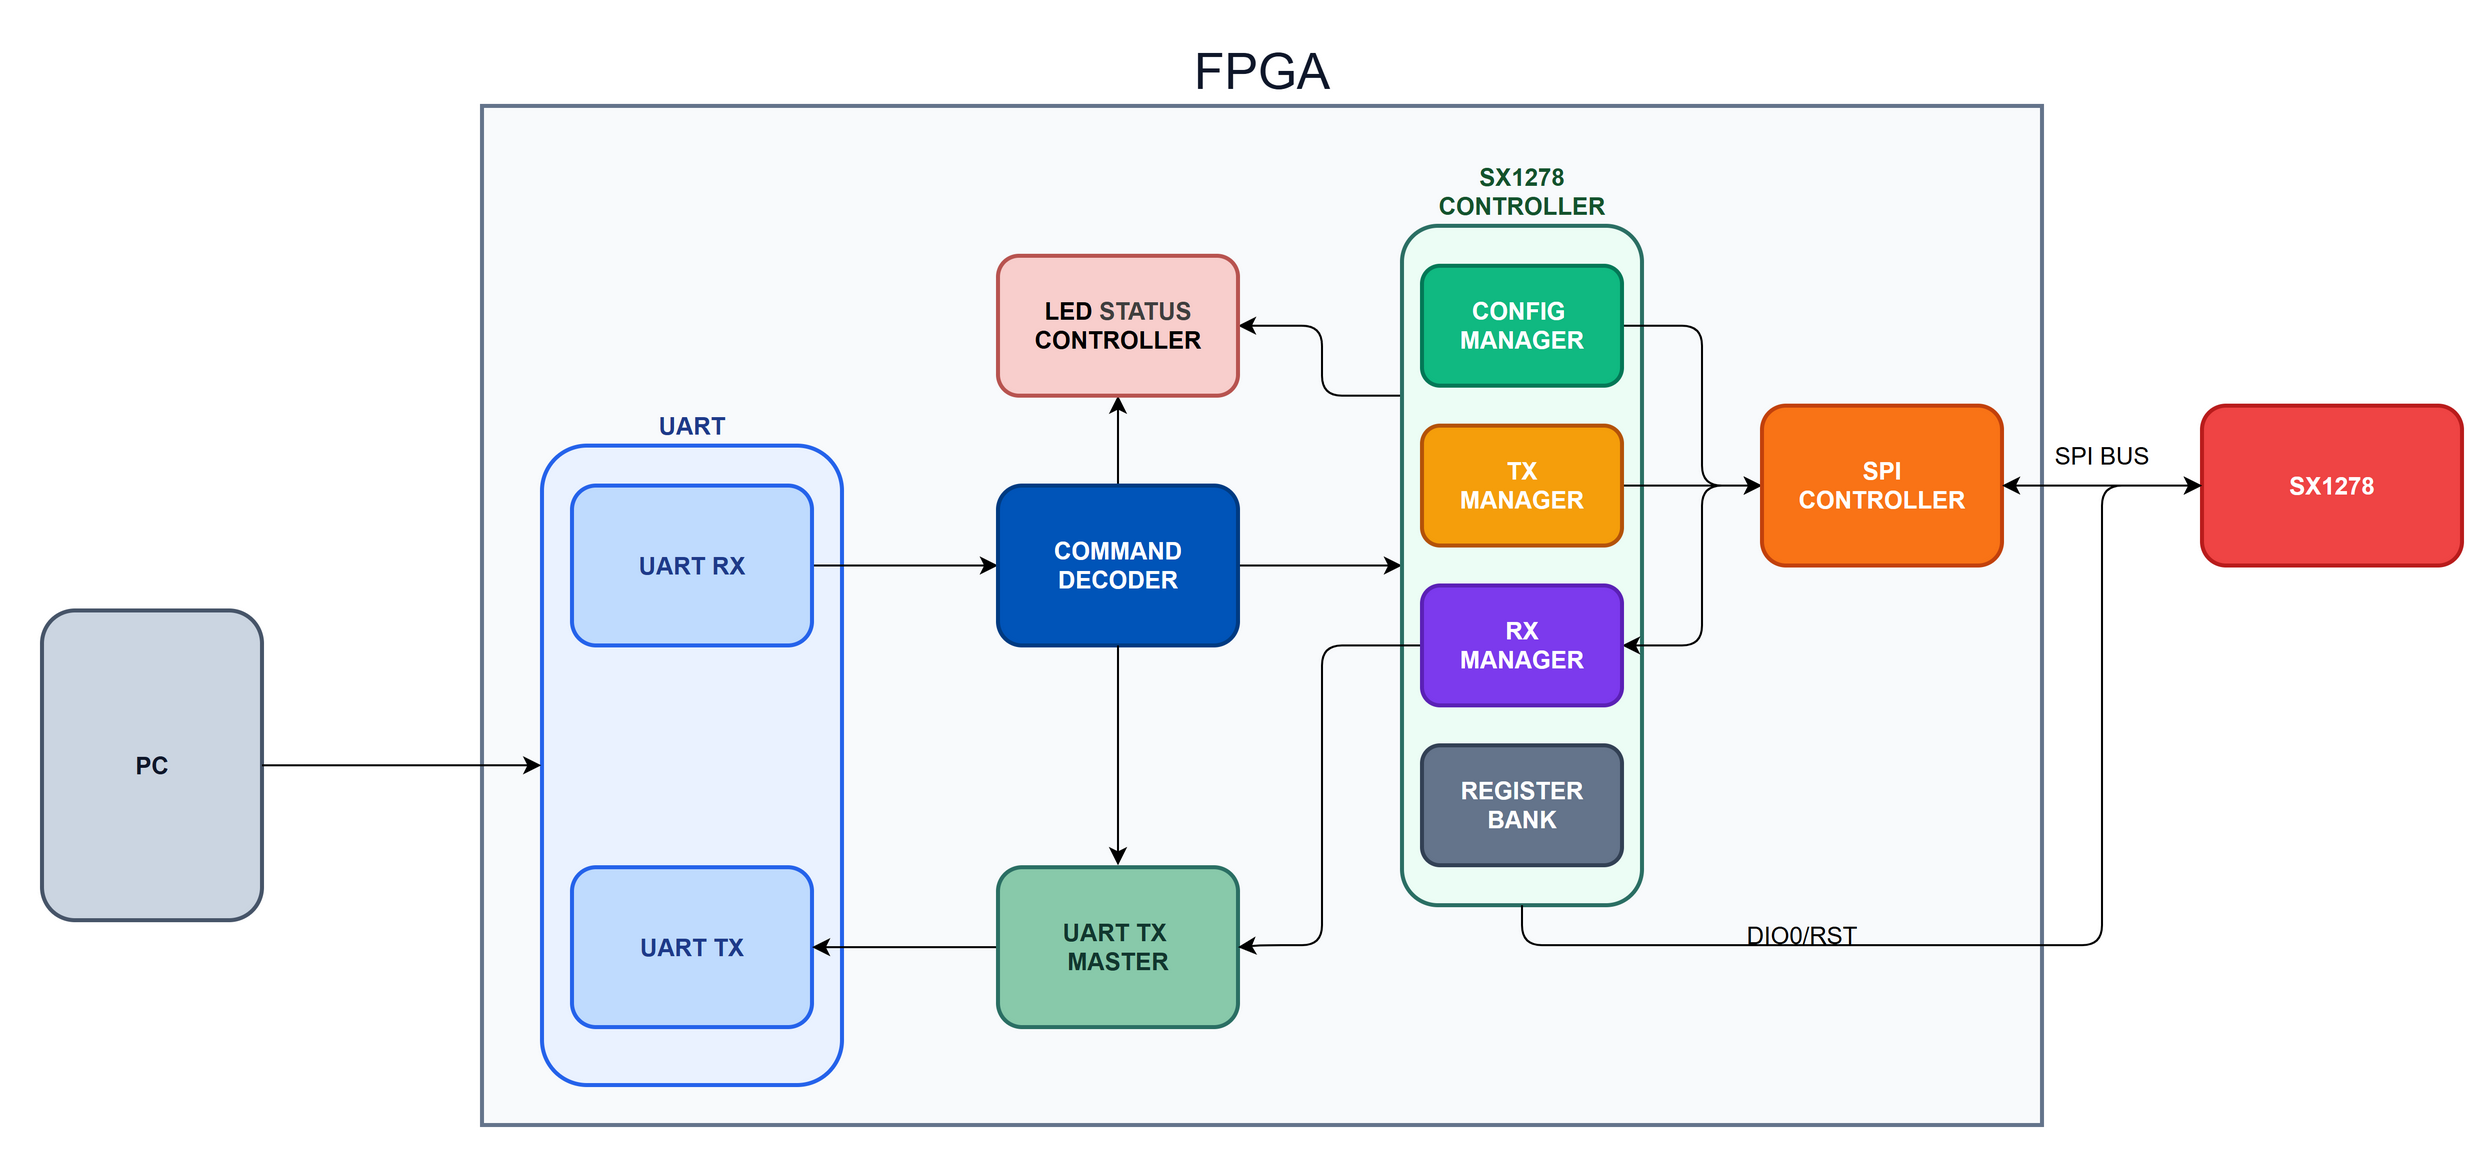
\includegraphics[width=\textwidth,height=0.71\textheight,keepaspectratio]{lora_top_arch.png}
    \caption{Diagrama en bloques del sistema completo.}
    \label{fig:top}
\end{figure}

\subsection{Flujo general}

\begin{enumerate}
    \item La UART reconstruye los bytes recibidos desde la PC.
    \item \module{command\_decoder} recibe una trama completa y verifica
          delimitadores, checksum, comando y parámetros.
    \item Si la orden es válida se genera un pulso hacia
          \module{sx1278\_controller}; de lo contrario se responde NACK.
    \item El controlador selecciona el manager de CONFIG, TX o RX.
    \item El manager solicita una secuencia al controlador SPI compartido.
    \item La cadena SPI convierte cada frame en \module{NSS}, \module{SCLK},
          \module{MOSI} y captura \module{MISO}.
    \item Las respuestas y los paquetes recibidos se serializan por UART.
\end{enumerate}

\newpage

\subsection{Interfaz UART y decoder de comandos}

La interfaz UART utiliza una trama de longitud fija:

\begin{lstlisting}
[#] [COMANDO] [PARAMETRO] [VALOR] [CHECKSUM] [$]
\end{lstlisting}

El checksum es el XOR de comando, parámetro y valor. El decoder espera la trama
completa antes de ejecutar una acción. Ante checksum, delimitador o comando
incorrecto responde NACK, permitiendo que el host reintente.

\begin{figure}[H]
    \centering
    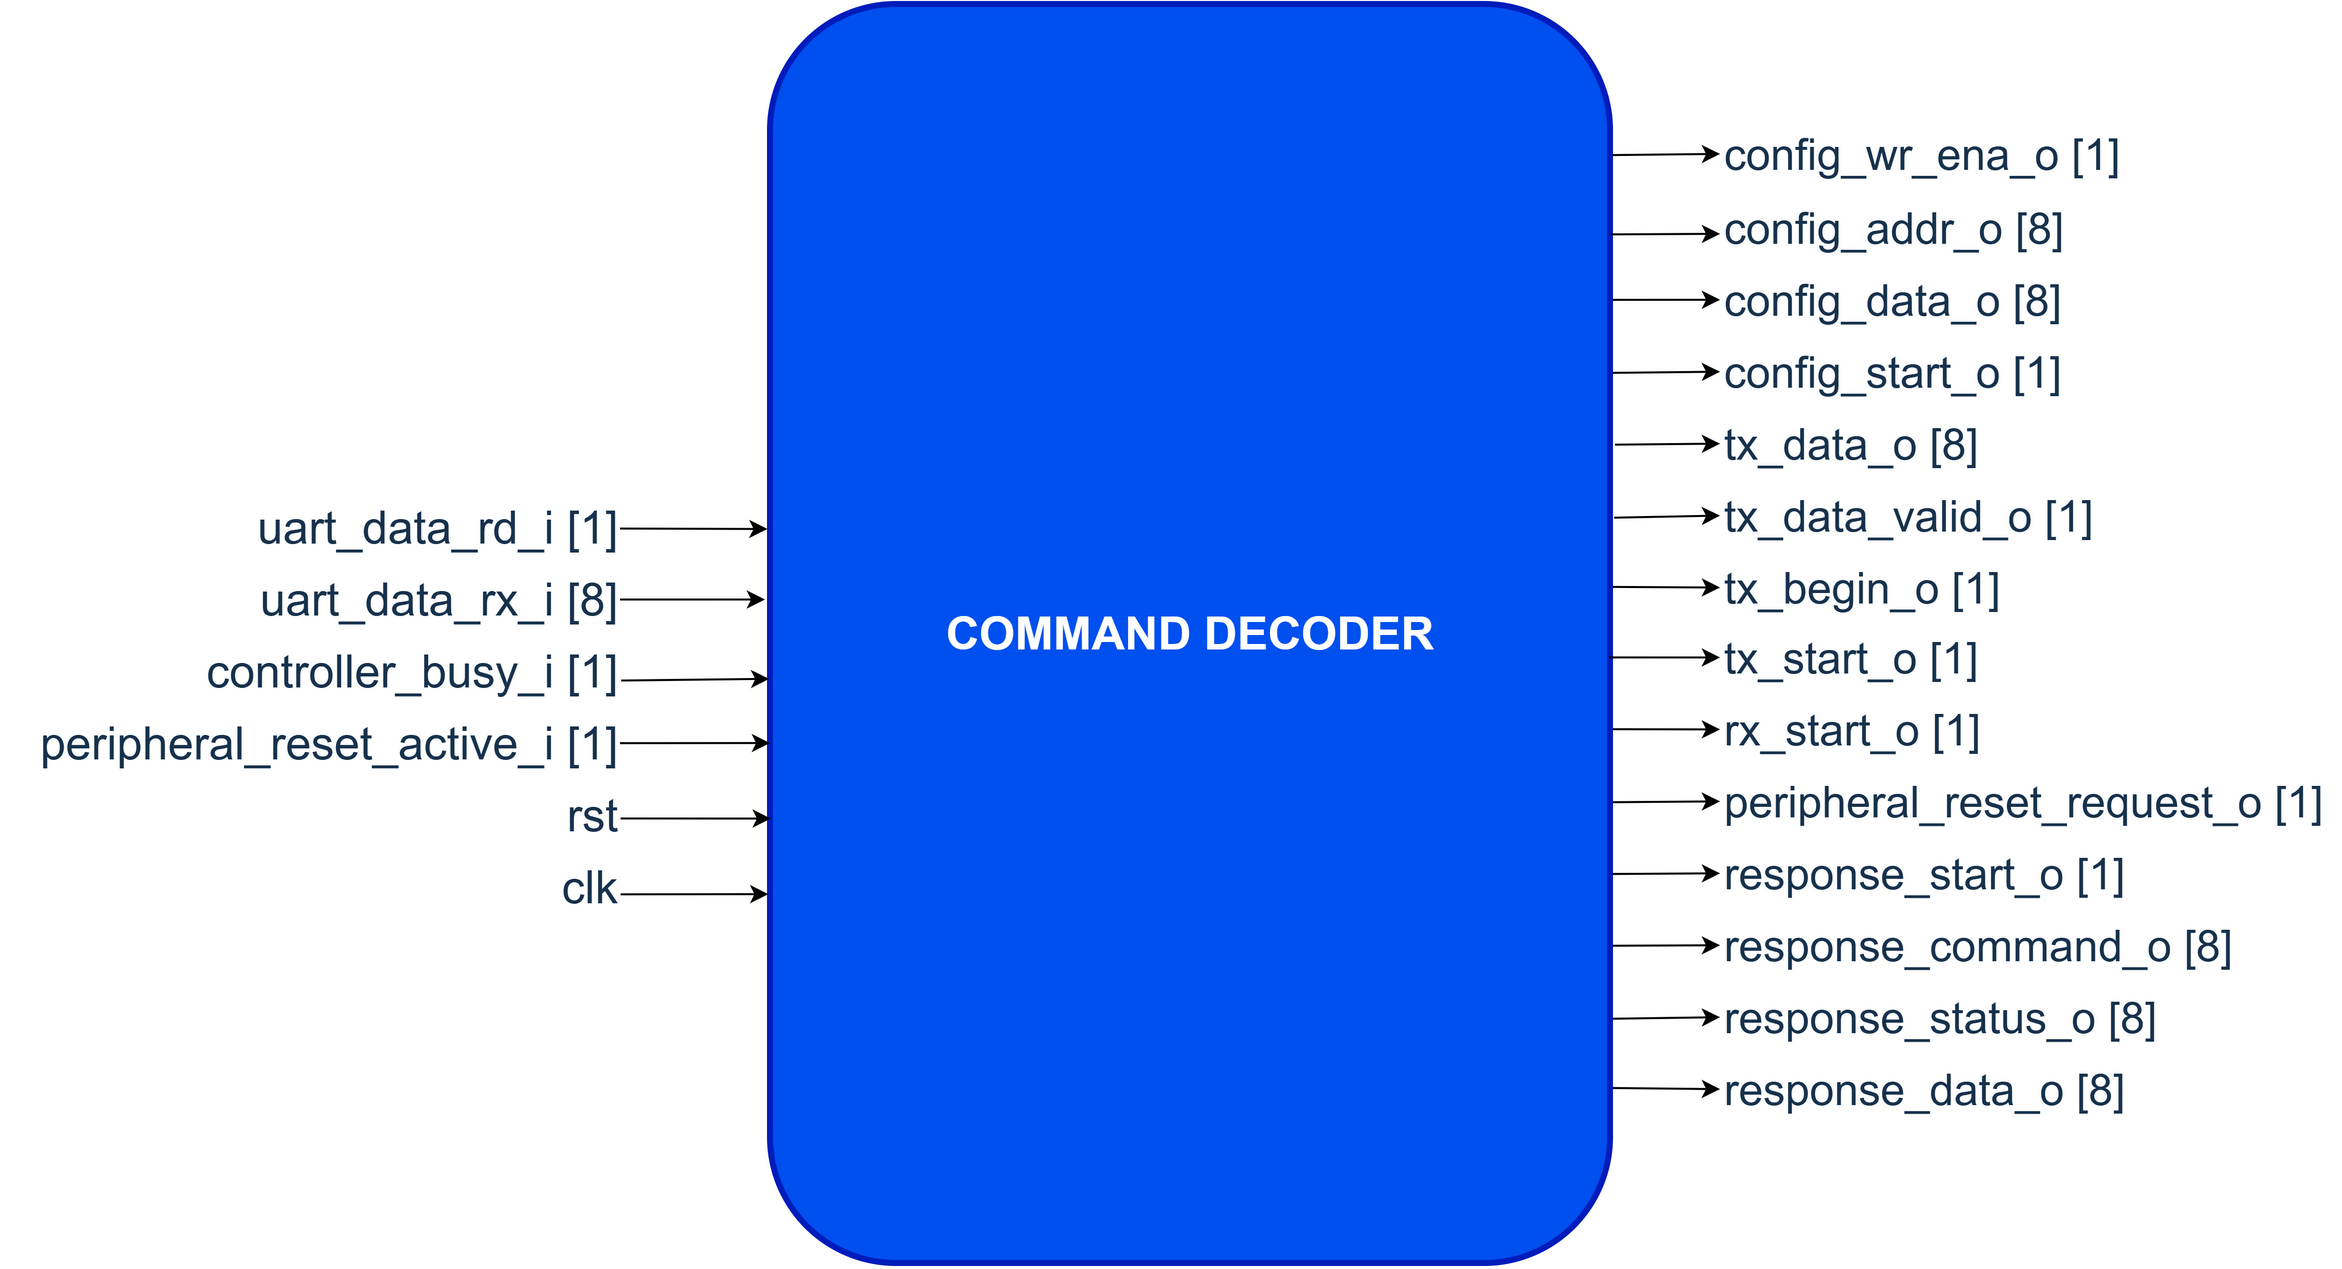
\includegraphics[width=0.94\textwidth,height=0.25\textheight,keepaspectratio]{command_decoder_interface.png}
    \caption{Interfaz del decoder de comandos UART.}
\end{figure}

\section{Controlador SX1278}

El controlador arbitra tres managers independientes. Todos comparten el mismo
secuenciador SPI y sólo uno puede solicitarlo en cada operación. La señal DIO0,
asíncrona respecto de \module{clk}, atraviesa un sincronizador y un detector de
flanco antes de ingresar a las máquinas de estado.

\subsection{Manager de configuración}

\module{sx1278\_config\_manager} recorre la secuencia de registros necesaria
para llevar el radio a LoRa, cargar los parámetros configurables, posicionar
las bases de FIFO y limpiar las interrupciones.

\begin{figure}[H]
    \centering
    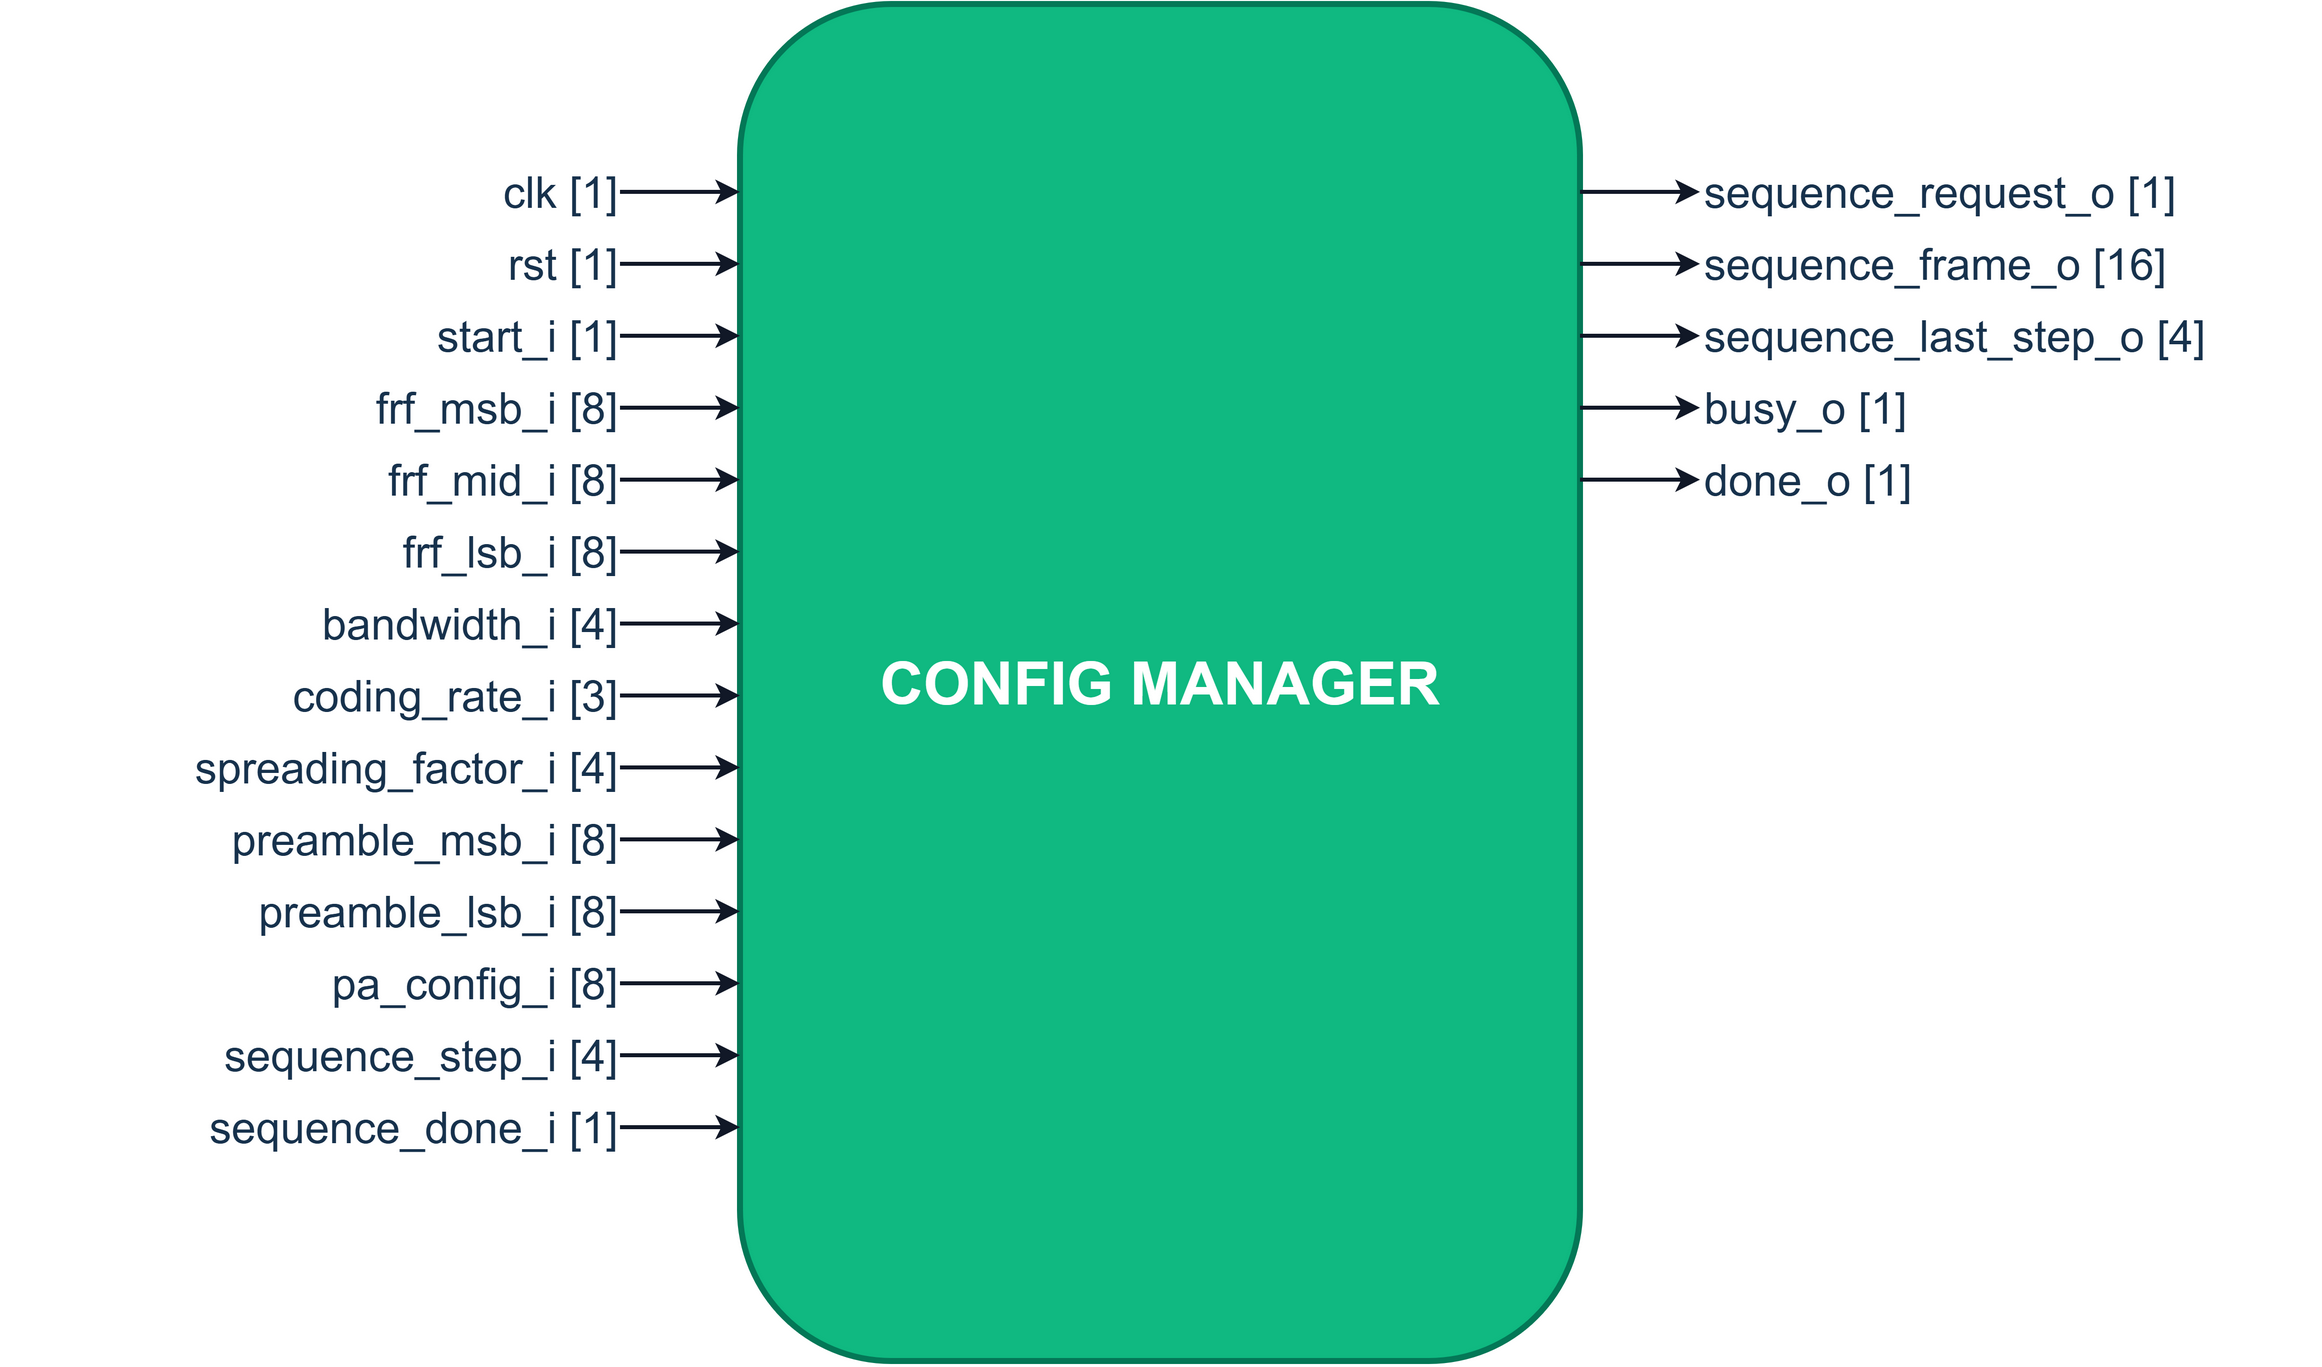
\includegraphics[width=\textwidth,height=0.25\textheight,keepaspectratio]{sx1278_config_manager_interface.png}
    \caption{Entradas y salidas del manager de configuración.}
\end{figure}

\subsection{Manager de transmisión}

\module{sx1278\_tx\_manager} mantiene un buffer local de hasta 50 bytes. Al
recibir la orden de transmisión prepara el puntero de FIFO, carga el payload,
programa la longitud, configura DIO0 como \module{TxDone}, inicia TX y espera
el flanco de DIO0.

\begin{figure}[H]
    \centering
    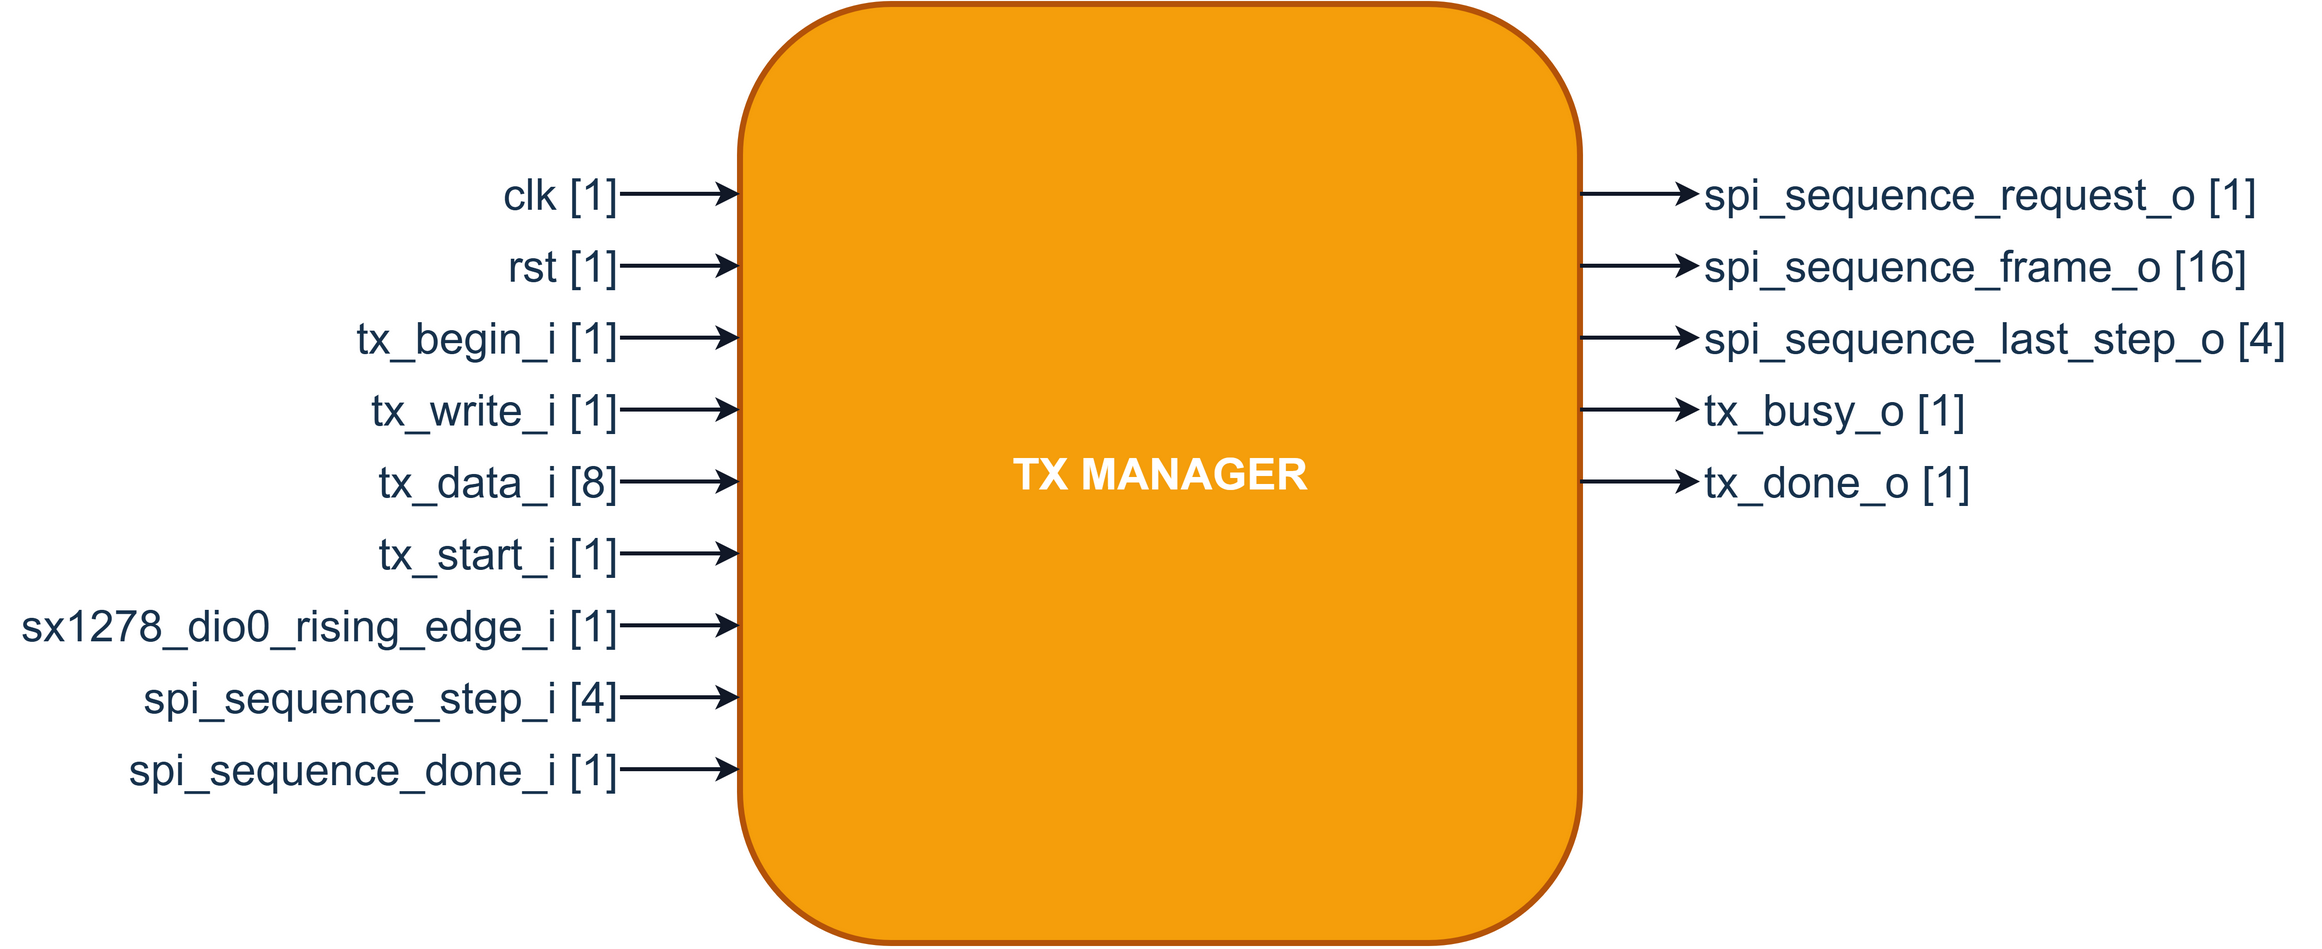
\includegraphics[width=\textwidth,height=0.57\textheight,keepaspectratio]{sx1278_tx_manager_interface.png}
    \caption{Entradas y salidas del manager de transmisión.}
\end{figure}

\subsection{Manager de recepción}

\module{sx1278\_rx\_manager} inicia el modo de recepción y espera DIO0. Luego
lee los flags IRQ, descarta paquetes con CRC incorrecto, obtiene longitud y
dirección de FIFO, almacena el payload y lo presenta al serializador UART.

\begin{figure}[H]
    \centering
    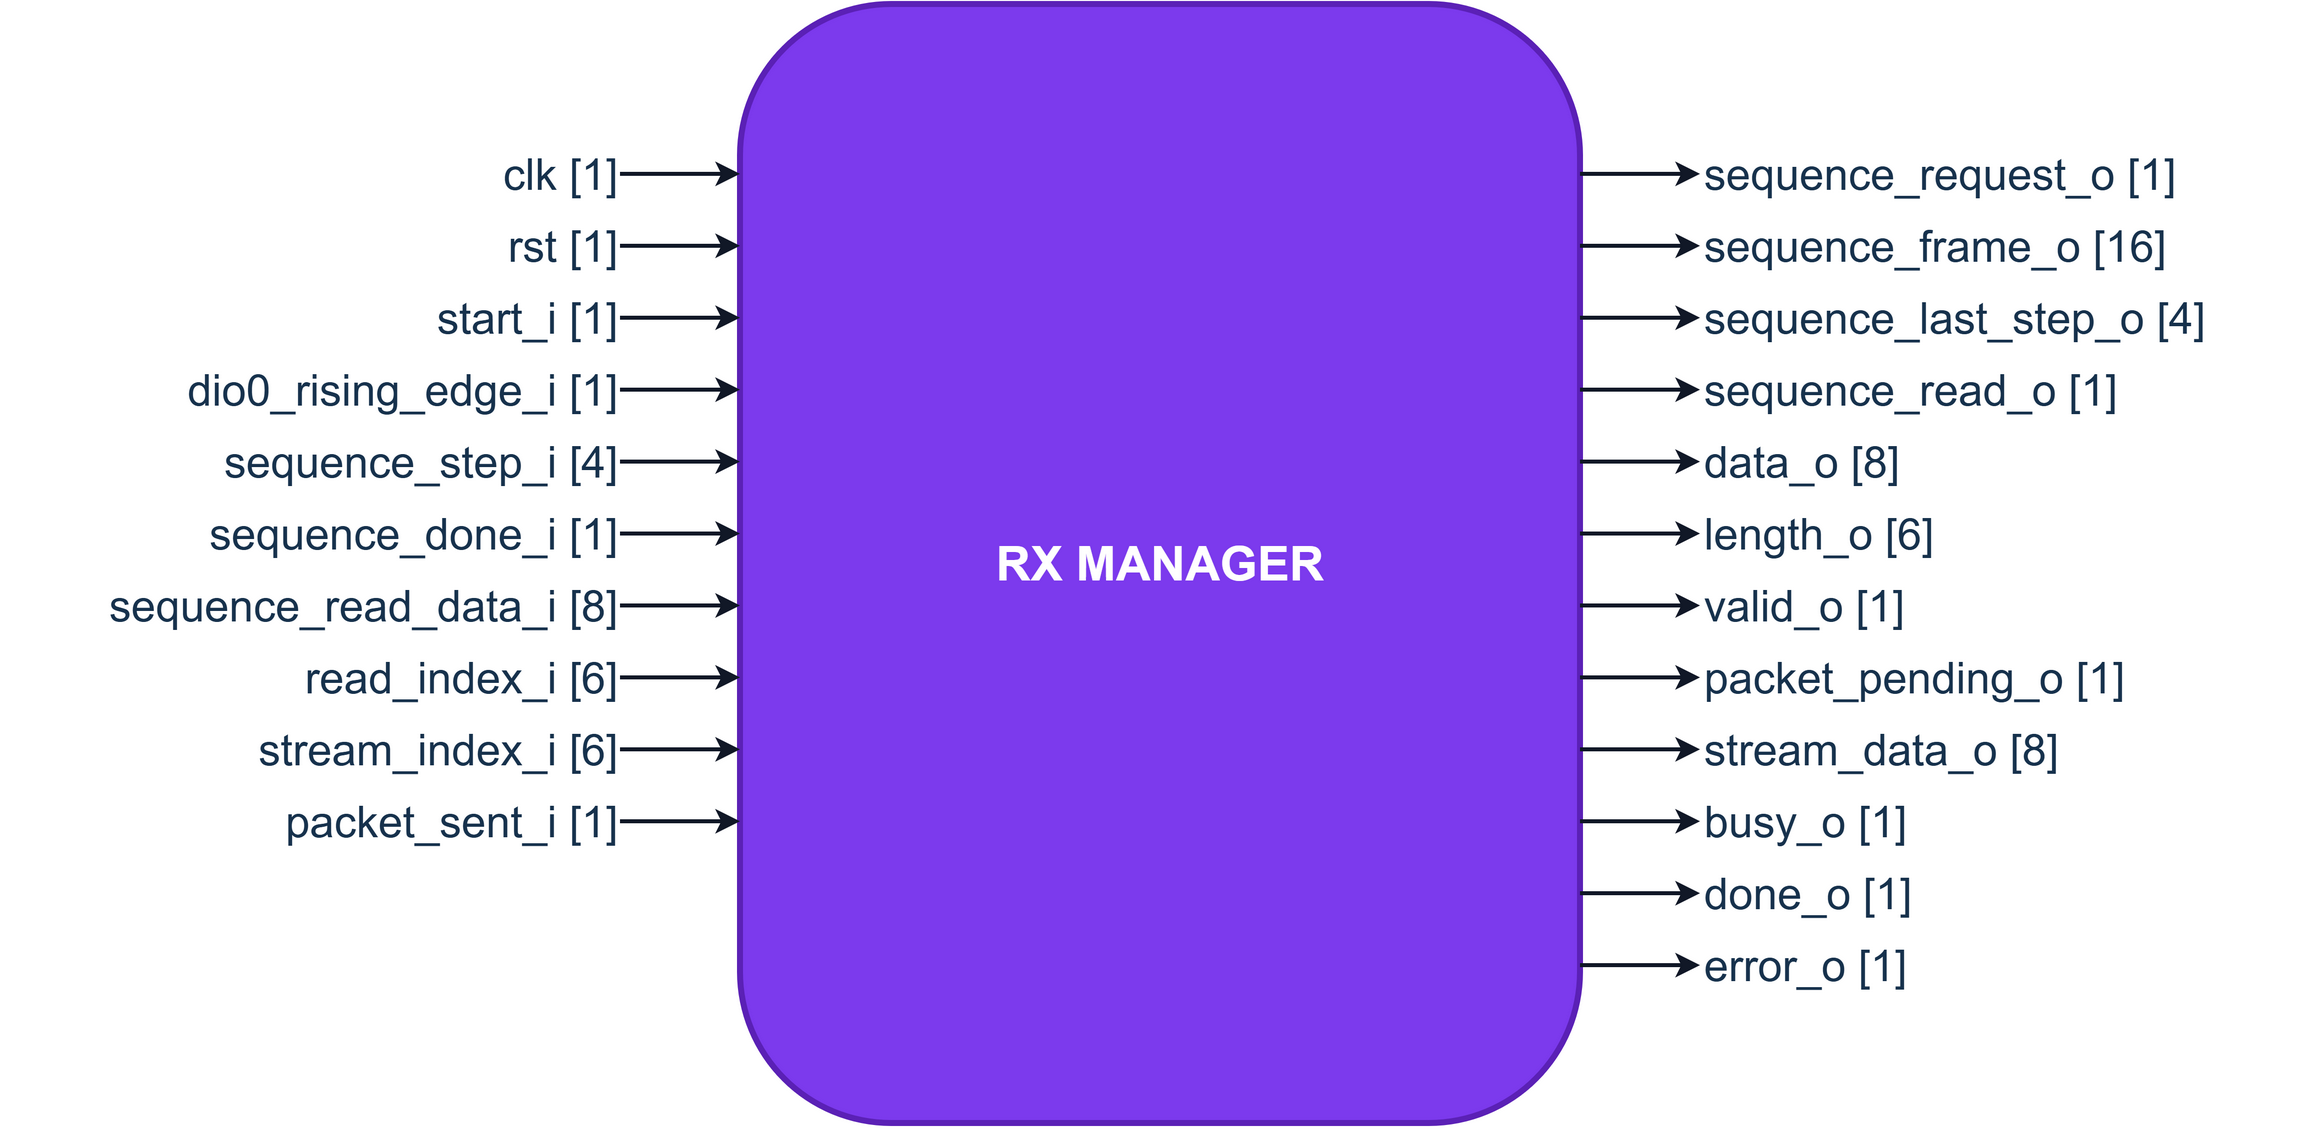
\includegraphics[width=\textwidth,height=0.62\textheight,keepaspectratio]{sx1278_rx_manager_interface.png}
    \caption{Entradas y salidas del manager de recepción.}
\end{figure}

\newpage
\section{Cadena SPI}

La cadena SPI se divide en tres niveles:

\begin{itemize}
    \item \module{spi\_sequence\_controller}: ejecuta una lista de accesos a
          registros.
    \item \module{spi\_register\_access}: adapta una lectura o escritura de
          registro a dos bytes SPI.
    \item \module{spi\_frame\_controller} y \module{spi\_pin\_driver}:
          almacenan los bytes, mantienen NSS durante el frame y generan o
          capturan las señales físicas.
\end{itemize}

Esta separación evita que las MEF de CONFIG, TX y RX tengan que generar flancos
de reloj o administrar directamente los bytes del bus.

\begin{figure}[H]
    \centering
    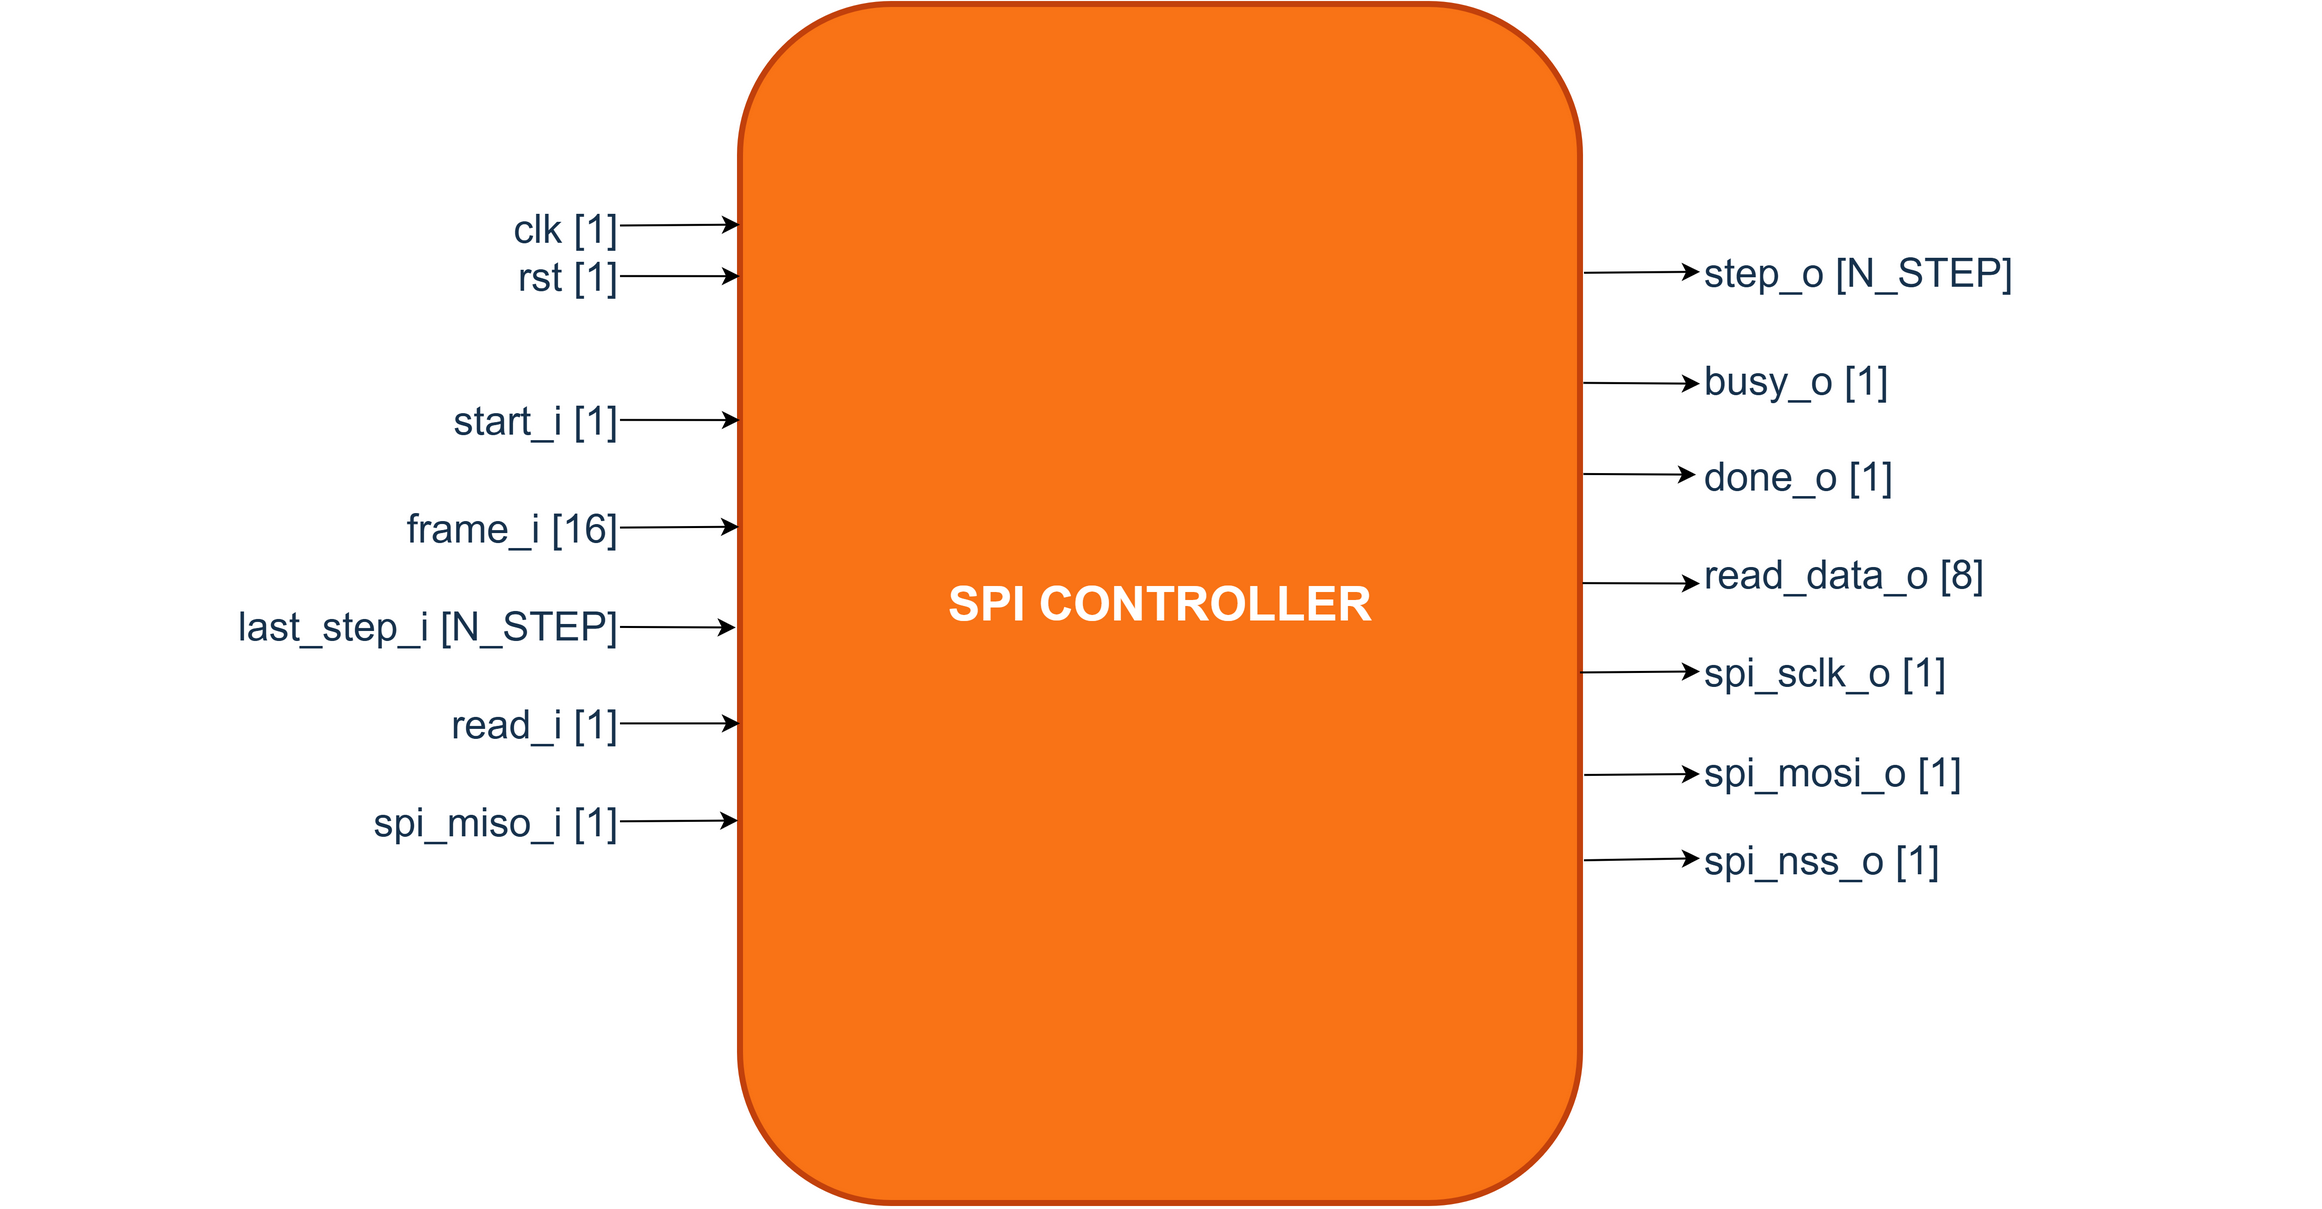
\includegraphics[width=0.96\textwidth,height=0.52\textheight,keepaspectratio]{spi_sequence_controller_interface.png}
    \caption{Interfaz del controlador de secuencias SPI.}
\end{figure}

\newpage

\section{Simulación y validación}

\subsection{Simulaciones realizadas}

La verificación se realizó en dos niveles. Los testbenches de componente
comprueban las interfaces básicas y el testbench del top comprueba el flujo
completo. De esta forma, los errores del protocolo UART o del bus SPI pueden
aislarse antes de ejecutar la integración.

\begin{table}[H]
    \centering
    \caption{Niveles de simulación utilizados.}
    \rowcolors{2}{lightGray}{white}
    \begin{tabularx}{\textwidth}{>{\raggedright\arraybackslash}p{0.27\textwidth}X}
        \toprule
        \textbf{Bloque verificado} & \textbf{Prueba principal} \\
        \midrule
        UART TX y UART RX & Transmisión y recepción de bytes individuales y secuencias de bytes a 115200 baud. \\
        SPI pin driver & Modos de polaridad y fase, datos \module{A5} y \module{81}, temporización de SCLK y muestreo de MISO. \\
        SPI frame controller & Carga de varios bytes, control de NSS, pausa entre bytes y captura de la respuesta. \\
        Decoder de comandos & Delimitadores, checksum XOR, ACK/NACK y generación de strobes de CONFIG, TX y RX. \\
        Controlador SX1278 & Secuencias de configuración, carga de TX, espera de DIO0 y recuperación del payload RX. \\
        Top completo & Comandos UART, actividad SPI, transmisión de payloads y devolución de un paquete recibido. \\
        \bottomrule
    \end{tabularx}
\end{table}

El testbench integrado \module{lora\_command\_fpga\_manager\_tb.vhd}
ejercita el camino completo UART--decoder--controlador--SPI. Las pruebas
principales son:

\begin{itemize}
    \item rechazo de checksum y delimitadores UART incorrectos;
    \item escritura y aplicación de configuración;
    \item transmisión de payloads mediante el SX1278;
    \item recepción y envío automático de los datos por UART.
\end{itemize}

Una ejecución correcta finaliza con:

\begin{lstlisting}
UART verificada: CONFIG, TX y RX automatico correctos
\end{lstlisting}

La Figura~\ref{fig:sim-top} presenta una ejecución del testbench de integración.
Se observan la actividad UART del host, las respuestas generadas por la FPGA,
el estado indicado por los LED y el comienzo de la actividad SPI.

\begin{figure}[H]
    \centering
    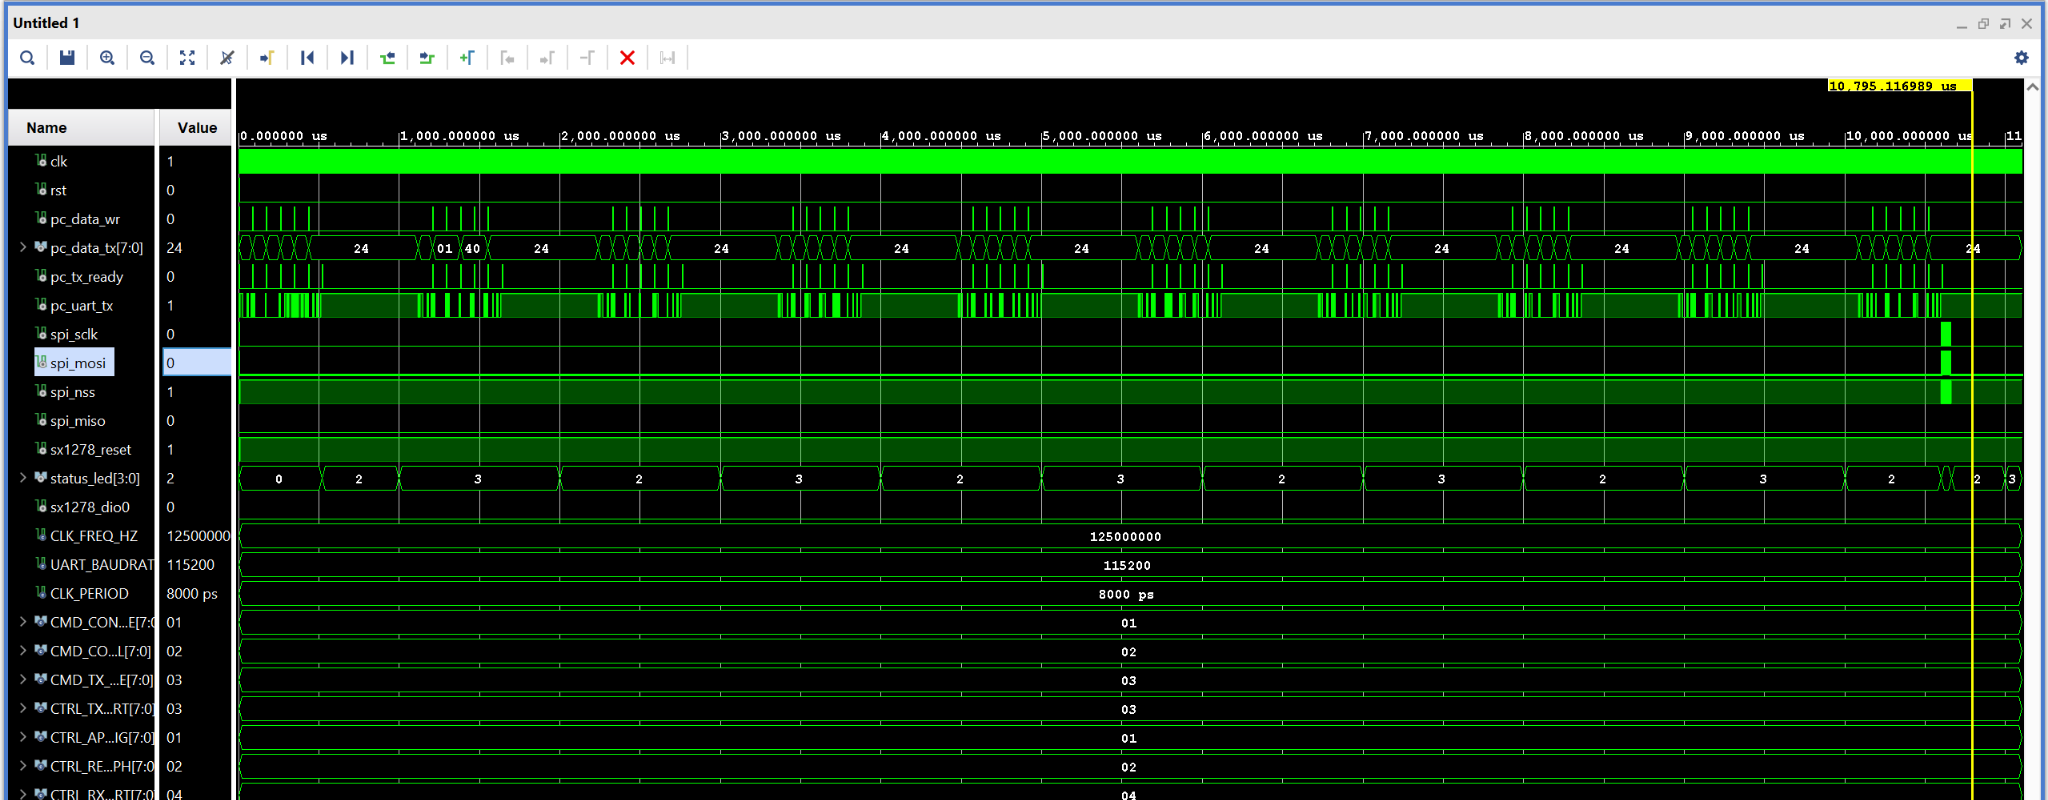
\includegraphics[width=\textwidth,height=0.43\textheight,keepaspectratio]{simulacion_top.png}
    \caption{Simulación del top completo en Vivado.}
    \label{fig:sim-top}
\end{figure}

\subsection{Validación sobre hardware}

El diseño se implementó sobre la FPGA Zynq y se conectó a un transceptor
SX1278. Como nodo LoRa complementario se utilizó una placa Heltec ESP32 LoRa,
mientras que un analizador lógico permitió observar las interfaces digitales
durante las pruebas. El montaje experimental se muestra en la
Figura~\ref{fig:montaje-hw}.

\begin{figure}[H]
    \centering
    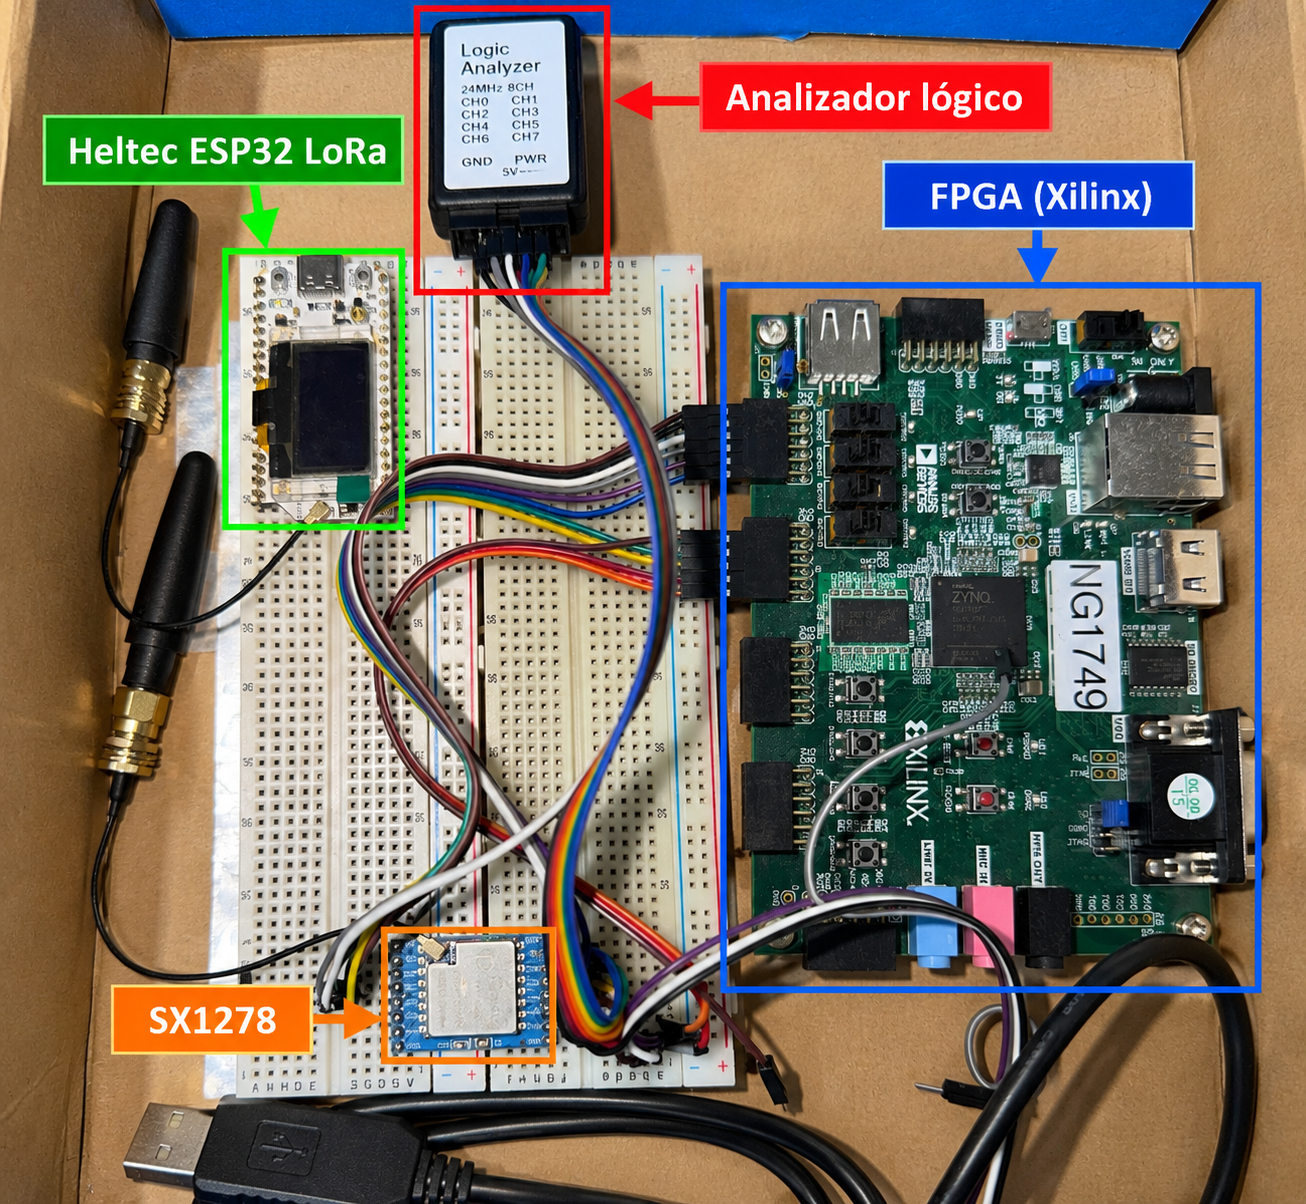
\includegraphics[width=0.82\textwidth,height=0.58\textheight,keepaspectratio]{montaje_validacion_hardware.png}
    \caption{Montaje experimental empleado para validar el controlador LoRa implementado en la FPGA.}
    \label{fig:montaje-hw}
\end{figure}

Además de verificar el intercambio LoRa, se observó el bus físico mediante el
analizador lógico. La Figura~\ref{fig:config-hw} muestra la secuencia SPI de
configuración y la Figura~\ref{fig:rx-hw} el inicio del modo de recepción.

\begin{figure}[H]
    \centering
    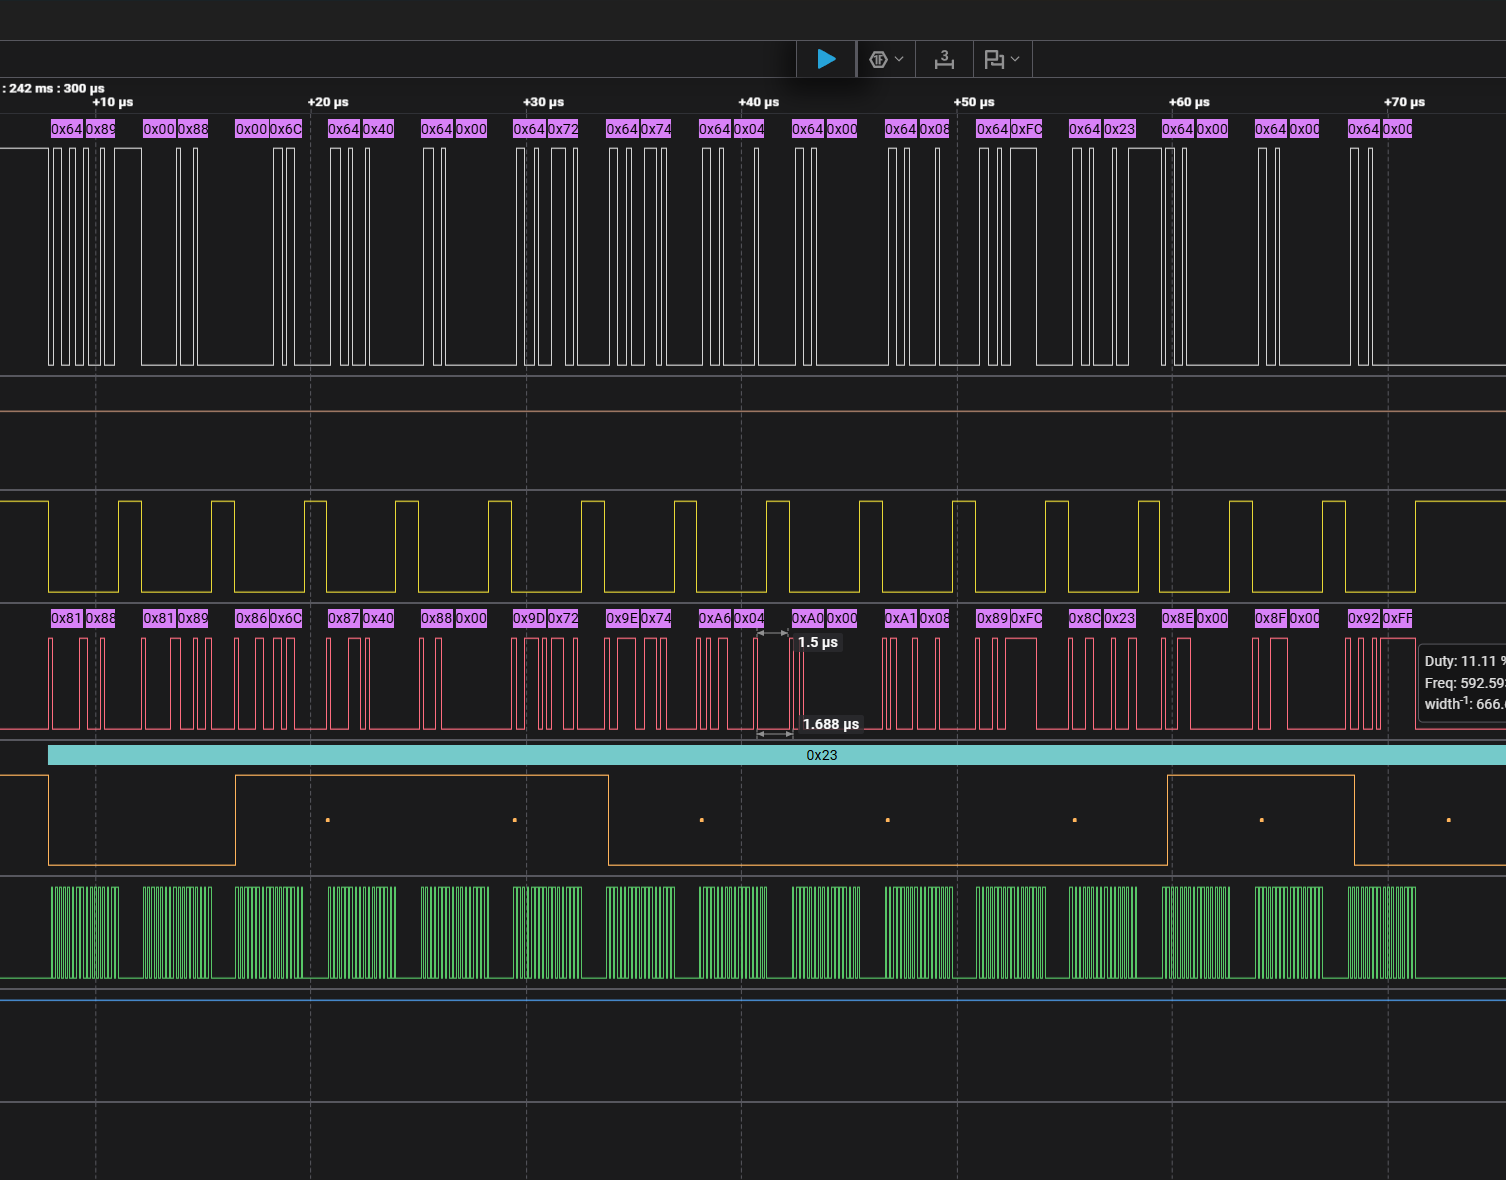
\includegraphics[width=\textwidth,height=0.48\textheight,keepaspectratio]{configuracion_spi_hardware.png}
    \caption{Secuencia SPI de configuración observada en hardware.}
    \label{fig:config-hw}
\end{figure}

\begin{figure}[H]
    \centering
    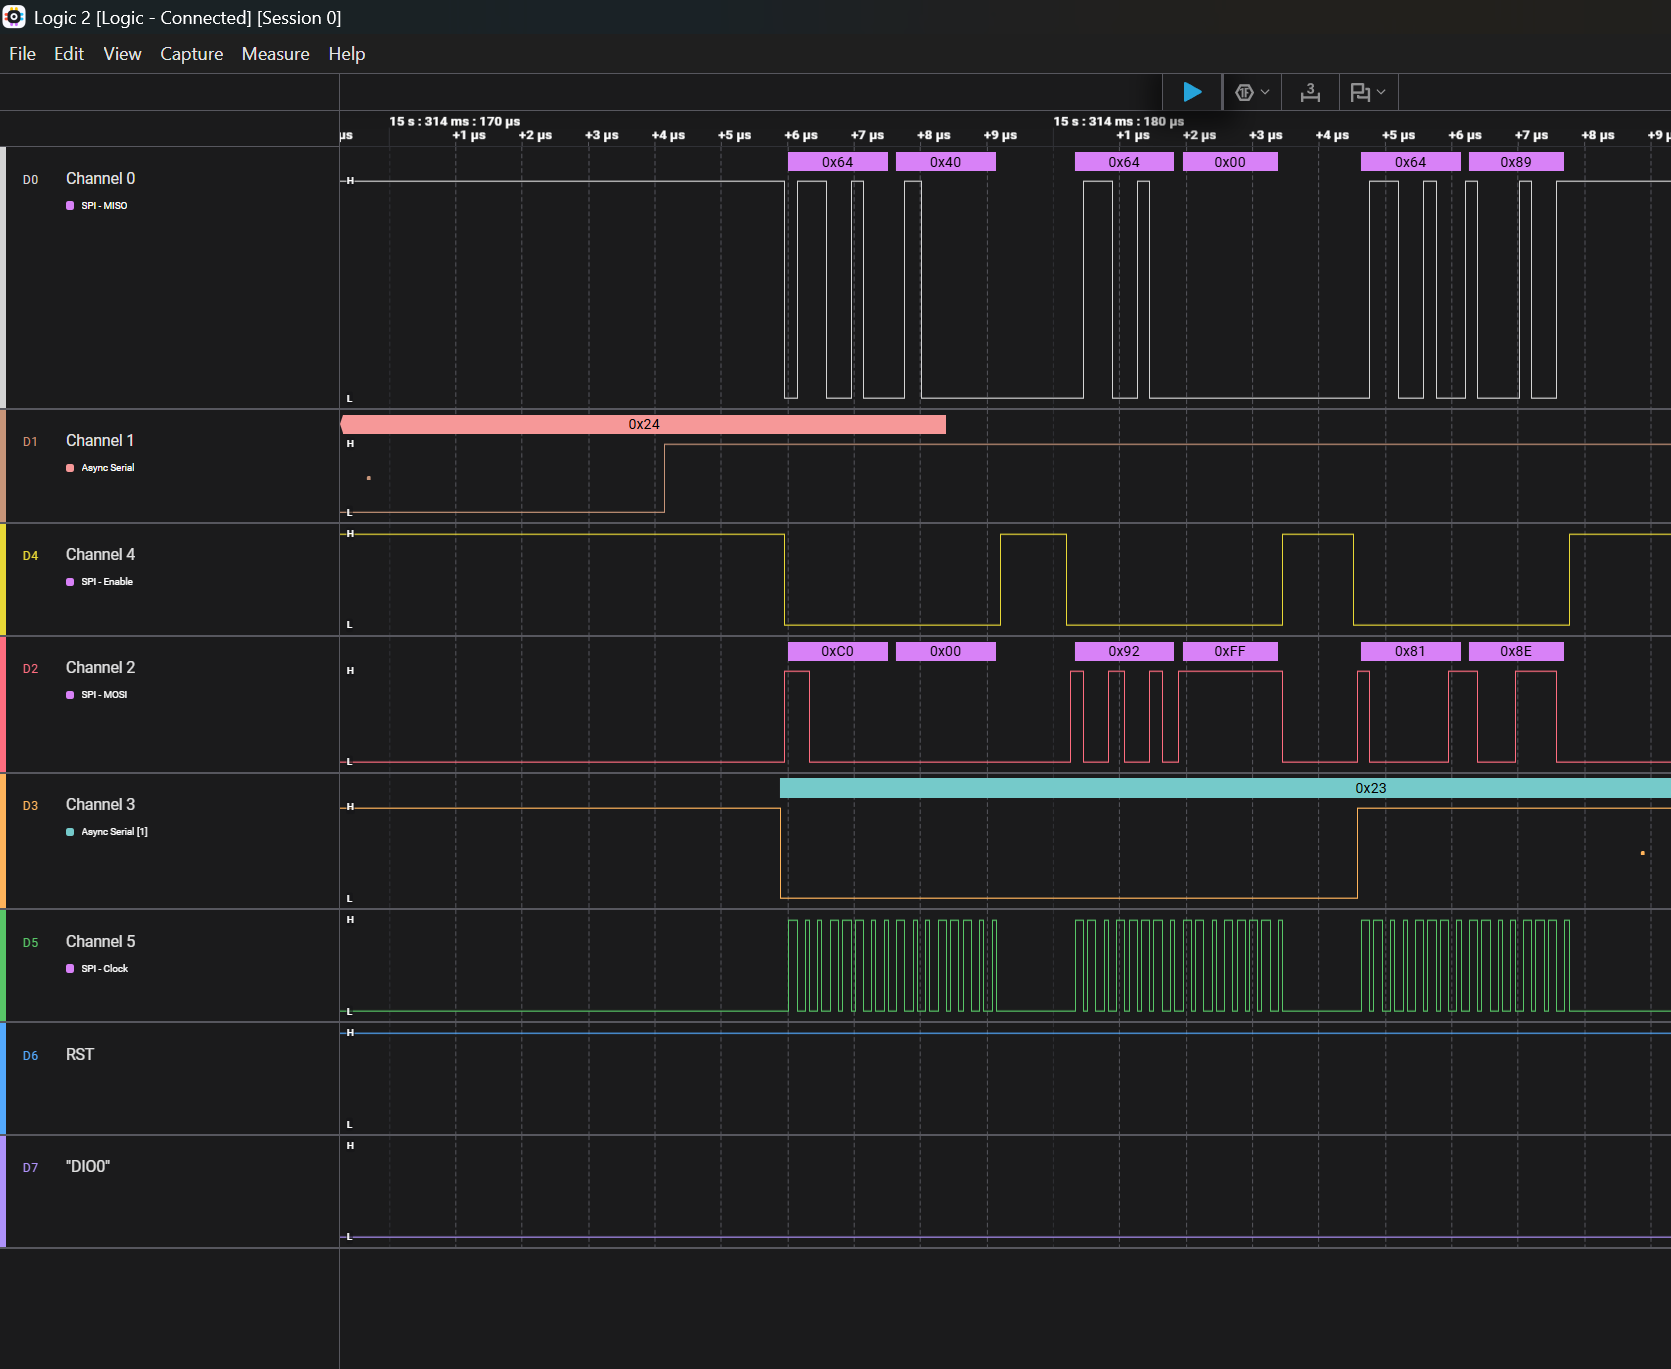
\includegraphics[width=\textwidth,height=0.48\textheight,keepaspectratio]{recepcion_spi_hardware.png}
    \caption{Configuración de DIO0, limpieza de IRQ e ingreso al modo RX.}
    \label{fig:rx-hw}
\end{figure}

Durante la integración se utilizó una separación de \textbf{20 ms} entre
comandos UART y hasta tres reintentos. Esta configuración permitió completar
transmisiones consecutivas sin superponer órdenes mientras el controlador se
encontraba ocupado.

\subsection{Síntesis, implementación y configuración de la FPGA}

Vivado sintetizó e implementó el top
\module{lora\_command\_fpga\_manager}. El flujo completó placement y ruteo,
generó los reportes de utilización y timing, y produjo el archivo de
configuración:

\begin{lstlisting}
LORA_FPGA.runs/impl_1/lora_command_fpga_manager.bit
\end{lstlisting}

El bitstream se descargó en la Zybo y el funcionamiento se comprobó con un
adaptador UART conectado a la PC, el módulo SX1278 y un analizador lógico. Las
capturas anteriores muestran las transacciones SPI obtenidas durante esa
validación.

\newpage

\section{Uso de recursos de la FPGA}

La Tabla~\ref{tab:resources} se obtuvo del reporte de utilización posterior a
placement de Vivado para el top \module{lora\_command\_fpga\_manager}.

\begin{table}[H]
    \centering
    \caption{Utilización de recursos de la Zybo Zynq-7000.}
    \label{tab:resources}
    \rowcolors{2}{lightGray}{white}
    \begin{tabular}{lrrr}
        \toprule
        \textbf{Recurso} & \textbf{Utilizado} & \textbf{Disponible} & \textbf{Utilización} \\
        \midrule
        Slice LUTs       & 851   & 17 600 & 4,84 \% \\
        Slice Registers  & 1 333 & 35 200 & 3,79 \% \\
        F7 Muxes         & 89    & 8 800  & 1,01 \% \\
        F8 Muxes         & 10    & 4 400  & 0,23 \% \\
        Block RAM Tile   & 0     & 60     & 0,00 \% \\
        DSP              & 0     & 80     & 0,00 \% \\
        Bonded IOB       & 14    & 100    & 14,00 \% \\
        BUFGCTRL         & 1     & 32     & 3,13 \% \\
        \bottomrule
    \end{tabular}
\end{table}

El diseño utiliza principalmente lógica distribuida y flip-flops. Las memorias
pequeñas destinadas a TX, RX y al frame SPI fueron implementadas por síntesis
sin consumir bloques BRAM dedicados.

\subsection{Resultado temporal}

\begin{table}[H]
    \centering
    \caption{Resumen temporal posterior al ruteo.}
    \rowcolors{2}{lightGray}{white}
    \begin{tabular}{lr}
        \toprule
        \textbf{Parámetro} & \textbf{Resultado} \\
        \midrule
        Frecuencia del reloj & 125 MHz \\
        Período               & 8,000 ns \\
        WNS                   & 0,280 ns \\
        TNS                   & 0,000 ns \\
        WHS                   & 0,139 ns \\
        THS                   & 0,000 ns \\
        \bottomrule
    \end{tabular}
\end{table}

Vivado informa que \textbf{todas las restricciones temporales definidas por el
usuario se cumplen}. Los datos completos se encuentran en los reportes
\path{lora_command_fpga_manager_utilization_placed.rpt} y
\path{lora_command_fpga_manager_timing_summary_routed.rpt}.

\section{Conclusiones}

El trabajo implementa una cadena completa de control LoRa en lógica
programable: recibe comandos de una PC, valida el protocolo, administra las
operaciones del SX1278 y genera el bus SPI. La división entre decoder, managers
y controladores físicos permite verificar cada módulo de manera aislada y
mantener las máquinas de estado enfocadas en una única responsabilidad.

La implementación ocupa menos del 5\,\% de las LUT y registros disponibles y
cumple timing a 125 MHz, dejando margen para incorporar nuevas funciones sin
cambiar la arquitectura principal.

Los secuenciadores dedicados fueron adecuados para el trabajo, aunque no
siempre son la alternativa más eficiente. Una evolución podría concentrar las
secuencias repetitivas en un \emph{IP core} AXI y delegar al procesador del SoC
Zynq la configuración y el control de alto nivel, simplificando las máquinas de
estado.

\end{document}
